%%%%%%%%%%%%%%%%%%%%%%%%%%%%%%%%%%%%%%%%%
% Twenty Seconds Resume/CV
% LaTeX Template
% Version 1.1 (8/1/17)
%
% This template has been downloaded from:
% http://www.LaTeXTemplates.com
%
% Original author:
% Carmine Spagnuolo (cspagnuolo@unisa.it) with major modifications by 
% Vel (vel@LaTeXTemplates.com)
%
% License:
% The MIT License (see included LICENSE file)
%
%%%%%%%%%%%%%%%%%%%%%%%%%%%%%%%%%%%%%%%%%

%----------------------------------------------------------------------------------------
%	PACKAGES AND OTHER DOCUMENT CONFIGURATIONS
%----------------------------------------------------------------------------------------

\documentclass[letterpaper]{twentysecondcv} % a4paper for A4

%----------------------------------------------------------------------------------------
%	 PERSONAL INFORMATION
%----------------------------------------------------------------------------------------

% If you don't need one or more of the below, just remove the content leaving the command, e.g. \cvnumberphone{}

\profilepic{carlpic.jpg} % Profile picture

\cvname{Carl Chittenden} % Your name
\cvjobtitle{Skier/Engineer} % Job title/career
\cvlinkedin{in/carl-chittenden-13a5a6aa}
\cvdate{6 April 1991} % Date of birth
\cvaddress{Bath, United Kingdom} % Short address/location, use \newline if more than 1 line is required
\cvnumberphone{+44 07816358232} % Phone number
\cvmail{carltc@hotmail.co.uk} % Email address

%----------------------------------------------------------------------------------------

\begin{document}

%----------------------------------------------------------------------------------------
%	 ABOUT ME
%----------------------------------------------------------------------------------------

\aboutme{I am half English and half Swedish ski enthusiast currently living in Bath, UK. I have been skiing for 12 years and snowboarding for 8 years pursuing my passion around the world in Canada, New Zealand, Sweden, France, Switzerland, Austria, Norway, Italy and the UK.} % To have no About Me section, just remove all the text and leave \aboutme{}

%----------------------------------------------------------------------------------------
%	 SKILLS
%----------------------------------------------------------------------------------------

% Skill bar section, each skill must have a value between 0 an 6 (float)
\skills{{German/3},{Swedish/5.8},{English/6}}

%------------------------------------------------

% Skill text section, each skill must have a value between 0 an 6
\skiskills{{Skiing - Level 11/11},{Snowboarding - Level 10/10}}

%----------------------------------------------------------------------------------------

\makeprofile % Print the sidebar

%----------------------------------------------------------------------------------------
%	 INTERESTS
%----------------------------------------------------------------------------------------

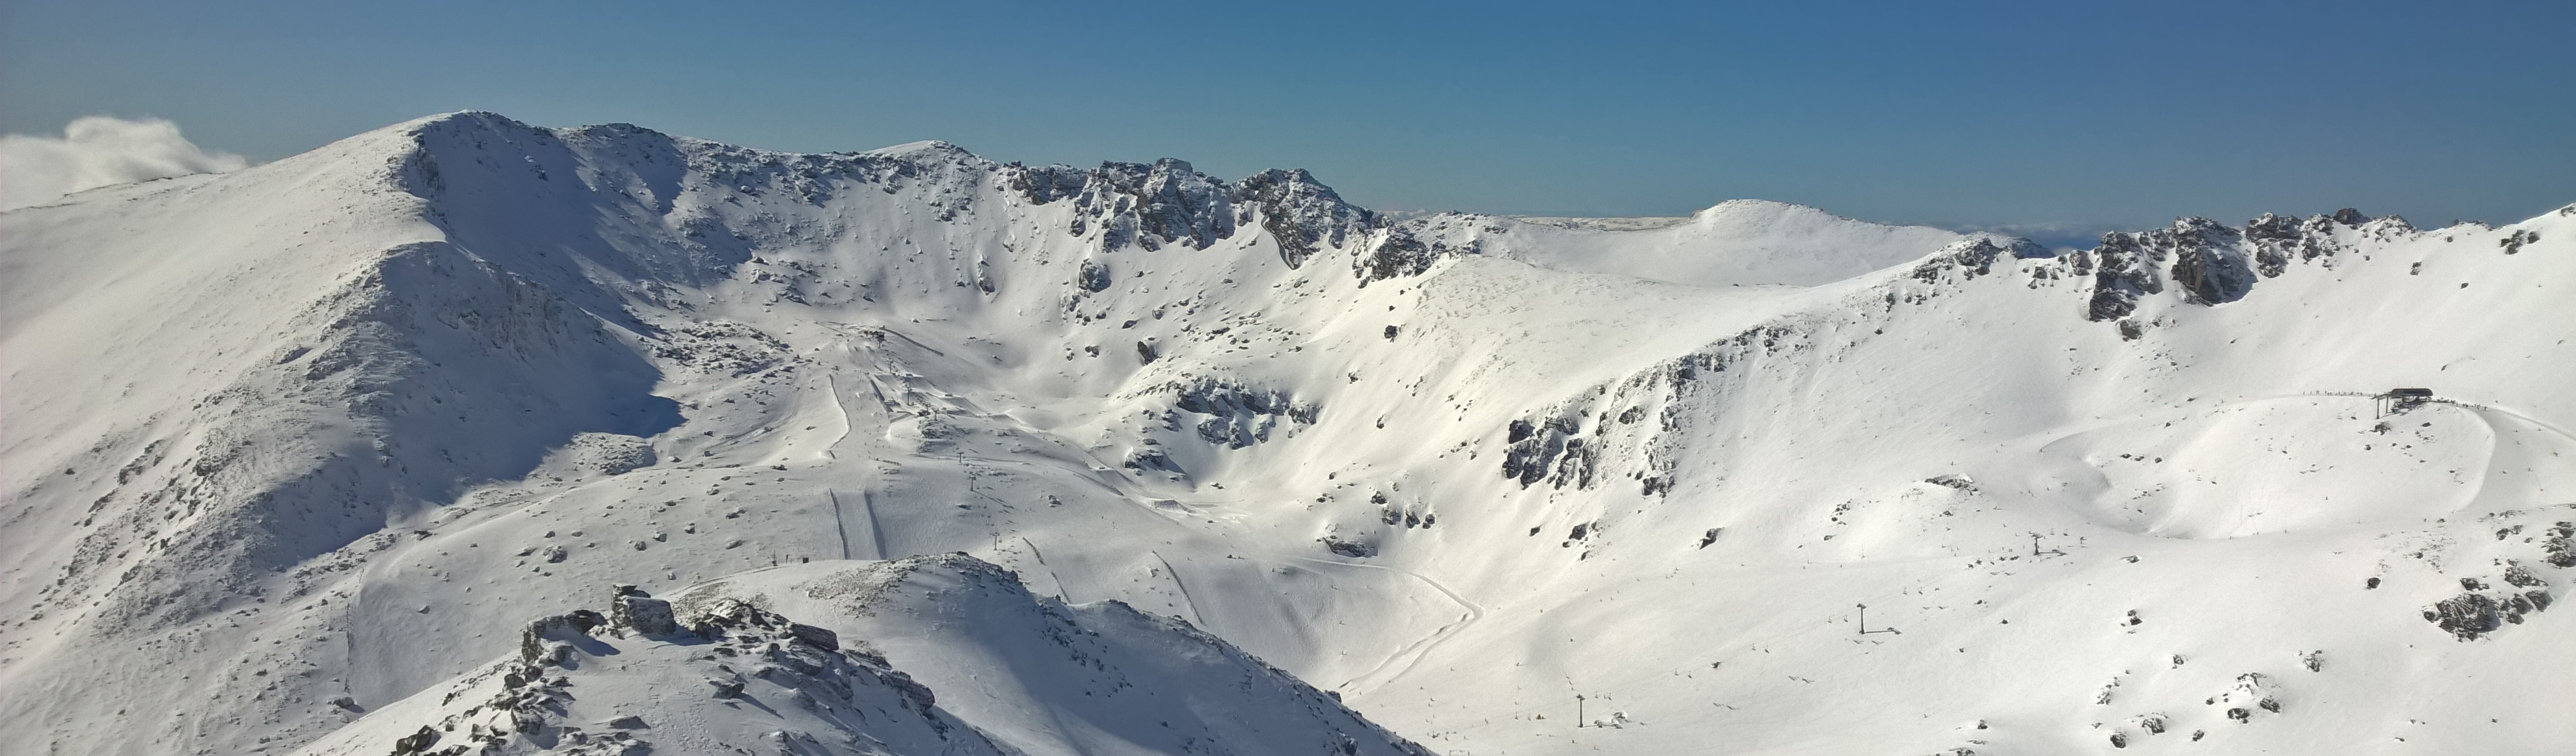
\includegraphics[width=\textwidth]{snowMountainsBanner.jpg}

\section{Bio}

In 2015 I went to New Zealand, became a qualified NZSIA Ski Instructor and worked a full season there in the ski school at Mt Hutt. During my time there I also learnt new skills such as ski maintenance and repair. After this I returned to the UK and went to university where I joined the Ski Race Team and competed for them at multiple competitions and trained regularly.

I have also kept my ski instructor skills sharp by teaching friends and family on trips each winter, taking beginners up to a level where they could confidently complete parallel turns and also honing skills of the already confident skiers.

I have now finished university and am looking for my next season location to work as an instructor. I am looking to complete my Snowboarding L1 qualification and also Ski L2 during my next season to continue my development as an instructor. I am already a very proficient snowboarder and improve and develop this alongside skiing.

%----------------------------------------------------------------------------------------
%	 EDUCATION
%----------------------------------------------------------------------------------------

\section{Education}

\begin{twenty} % Environment for a list with descriptions
	\twentyitemmedium{2015 - 2018}{Ph.D. {\normalfont in Electrical Engineering}}{University of Bath, UK}
	\twentyitemmedium{2009-2014}{M.Eng. Mechanical and Electrical Engineering}{University of Bath, UK}
	%\twentyitem{<dates>}{<title>}{<location>}{<description>}
\end{twenty}


%----------------------------------------------------------------------------------------
%	 Qualifications
%----------------------------------------------------------------------------------------

\section{Qualifications}

\begin{twentyshort} % Environment for a short list with no descriptions
    \twentyitemacross{2015}{Ski Instructor L1}{
\includegraphics[height=0.05\textwidth]{NZSIA-Logo.png}}{New Zealand}
	%\twentyitemshort{<dates>}{<title/description>}
\end{twentyshort}

%----------------------------------------------------------------------------------------
%	 EXPERIENCE
%----------------------------------------------------------------------------------------

\section{Professional Experience}

\begin{twenty} % Environment for a list with descriptions
	\twentyitemacross{2015}{Ski Instructor}{
\includegraphics[height=0.05\textwidth]{nzskilogo.png}}{Mt Hutt, New Zealand}
	%\twentyitem{<dates>}{<title>}{<location>}{<description>}
\end{twenty}

\section{Experience}

\begin{twenty} % Environment for a list with descriptions
	\twentyitemacross{2015 - 2017}{Ski Race Team}{
\includegraphics[height=0.05\textwidth]{bathSnowsports.jpg} \hspace{0.5cm} Bath Snowsports}{Bath, UK}
	%\twentyitem{<dates>}{<title>}{<location>}{<description>}
\end{twenty}

  \section{Photos}
  \subsection{NZSki, Mt Hutt - Ski Instructor}
      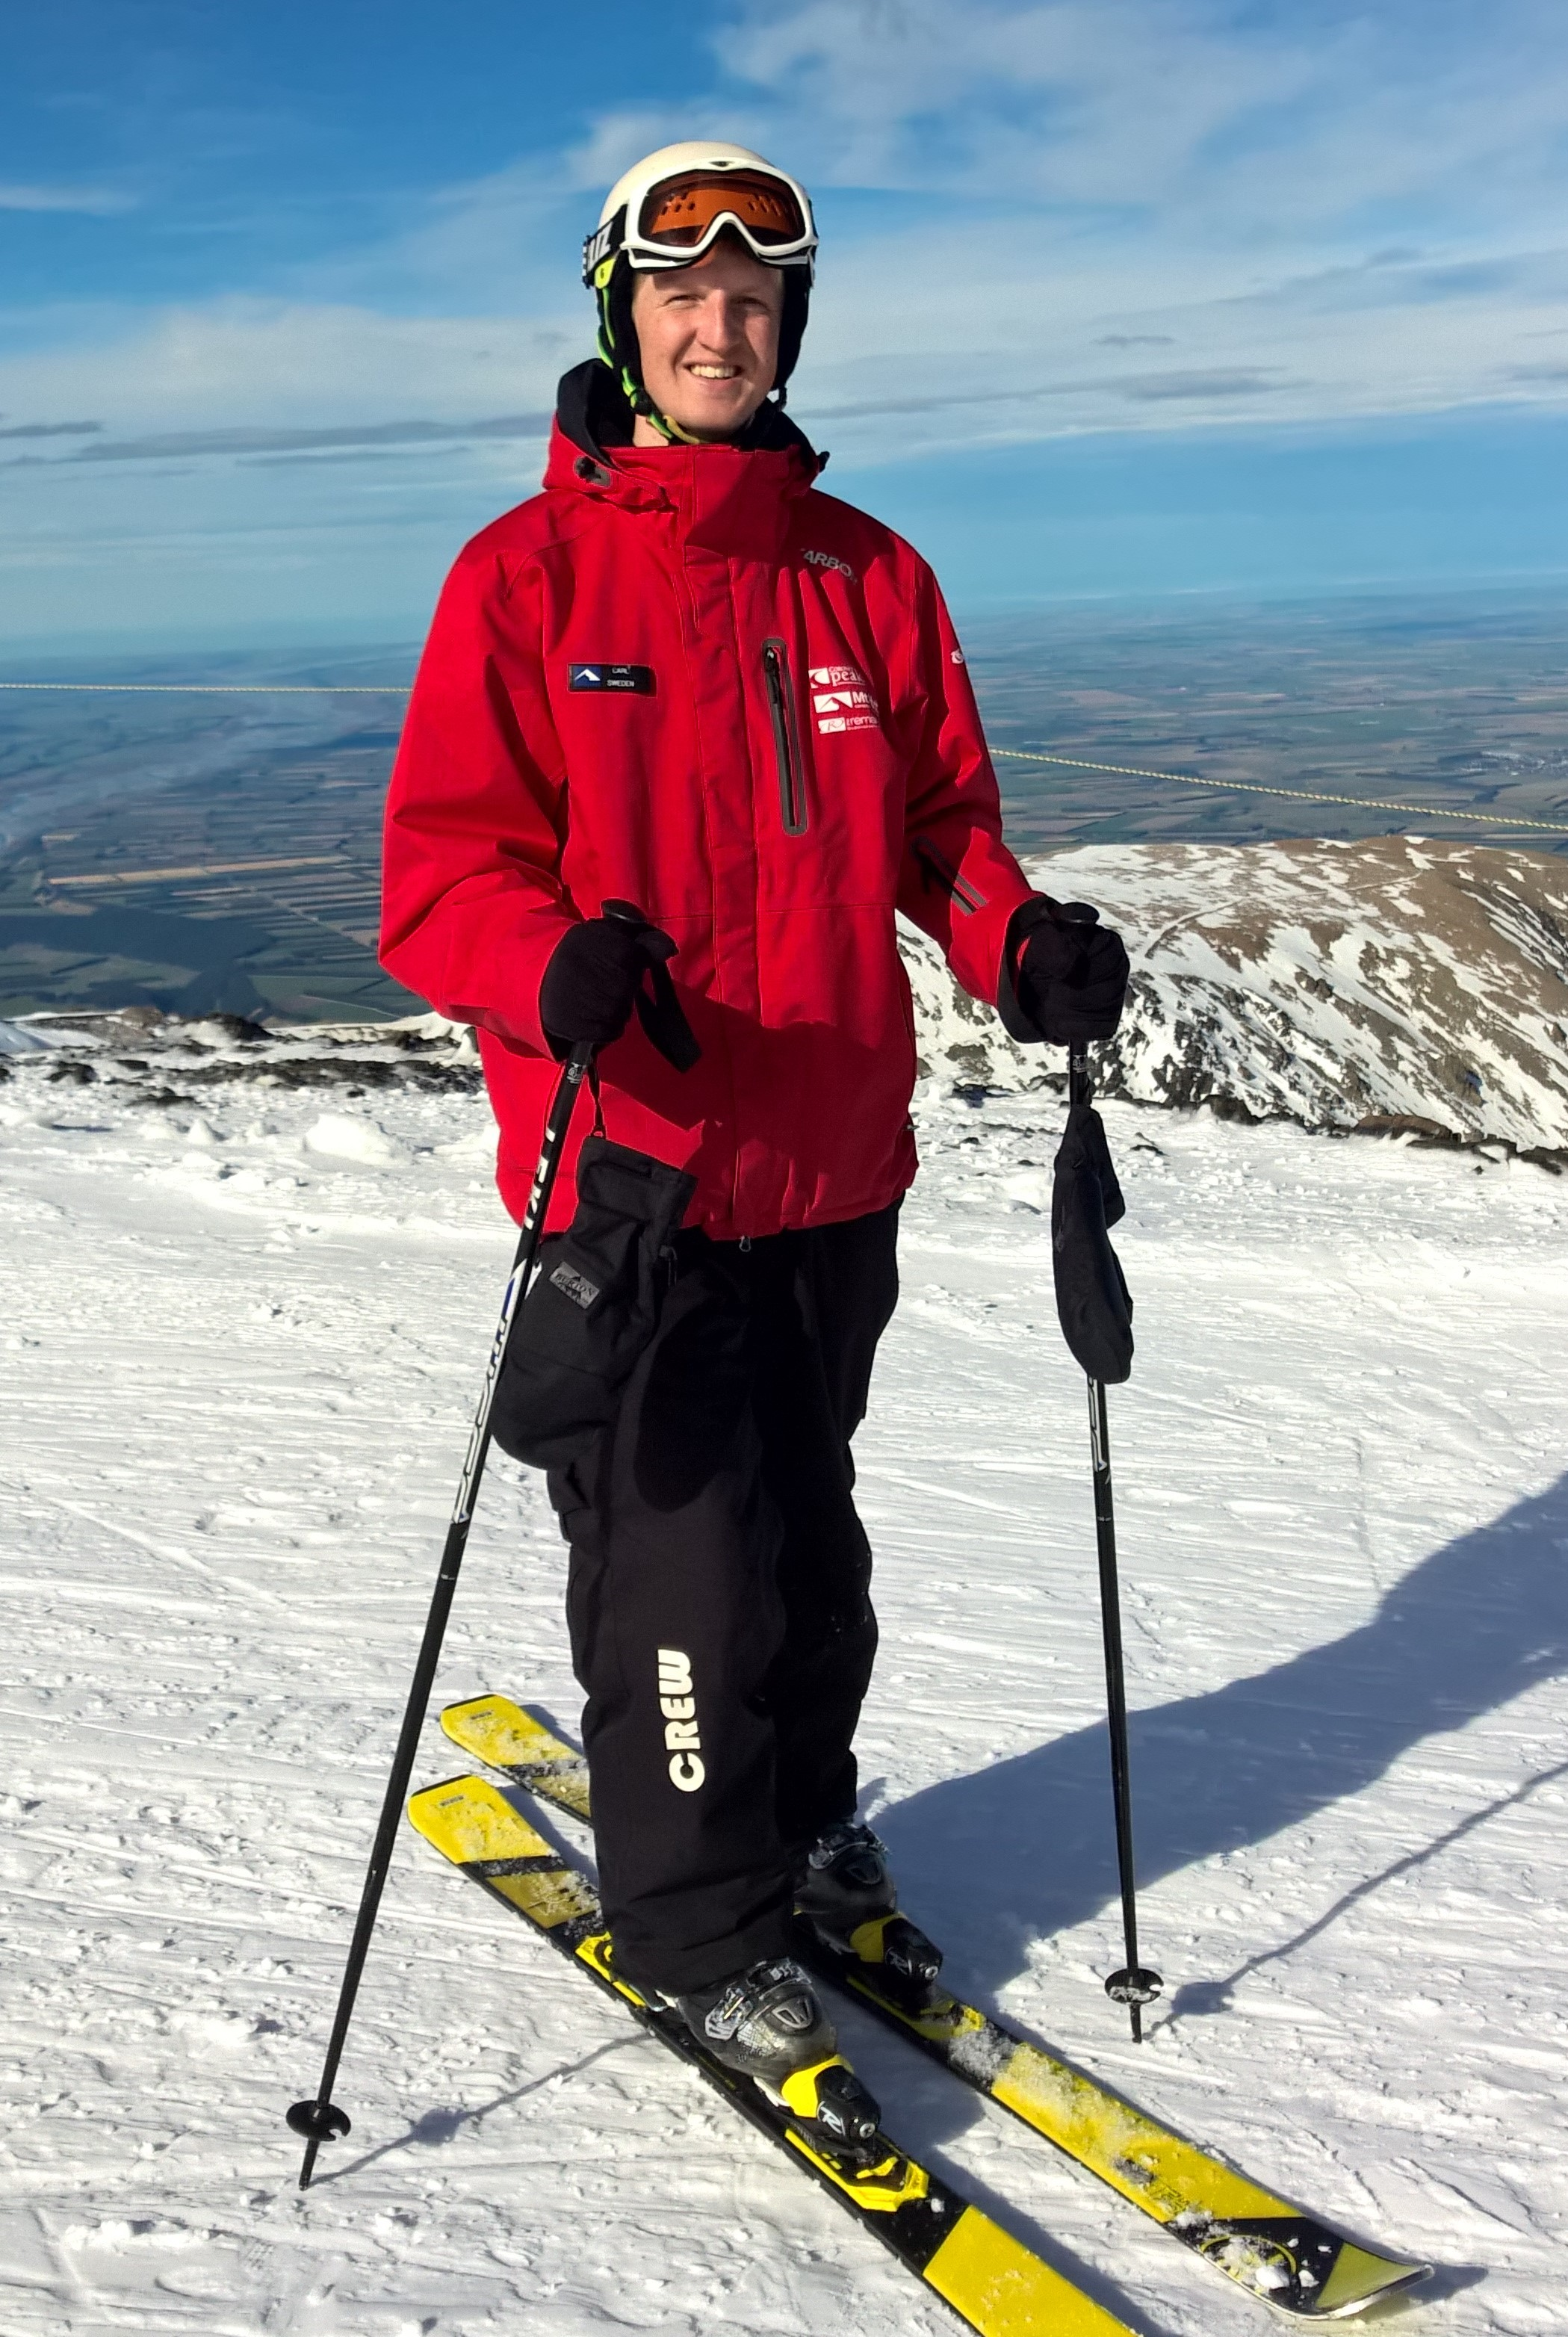
\includegraphics[height=0.4\textwidth]{skiInstructorPicture.jpg}
      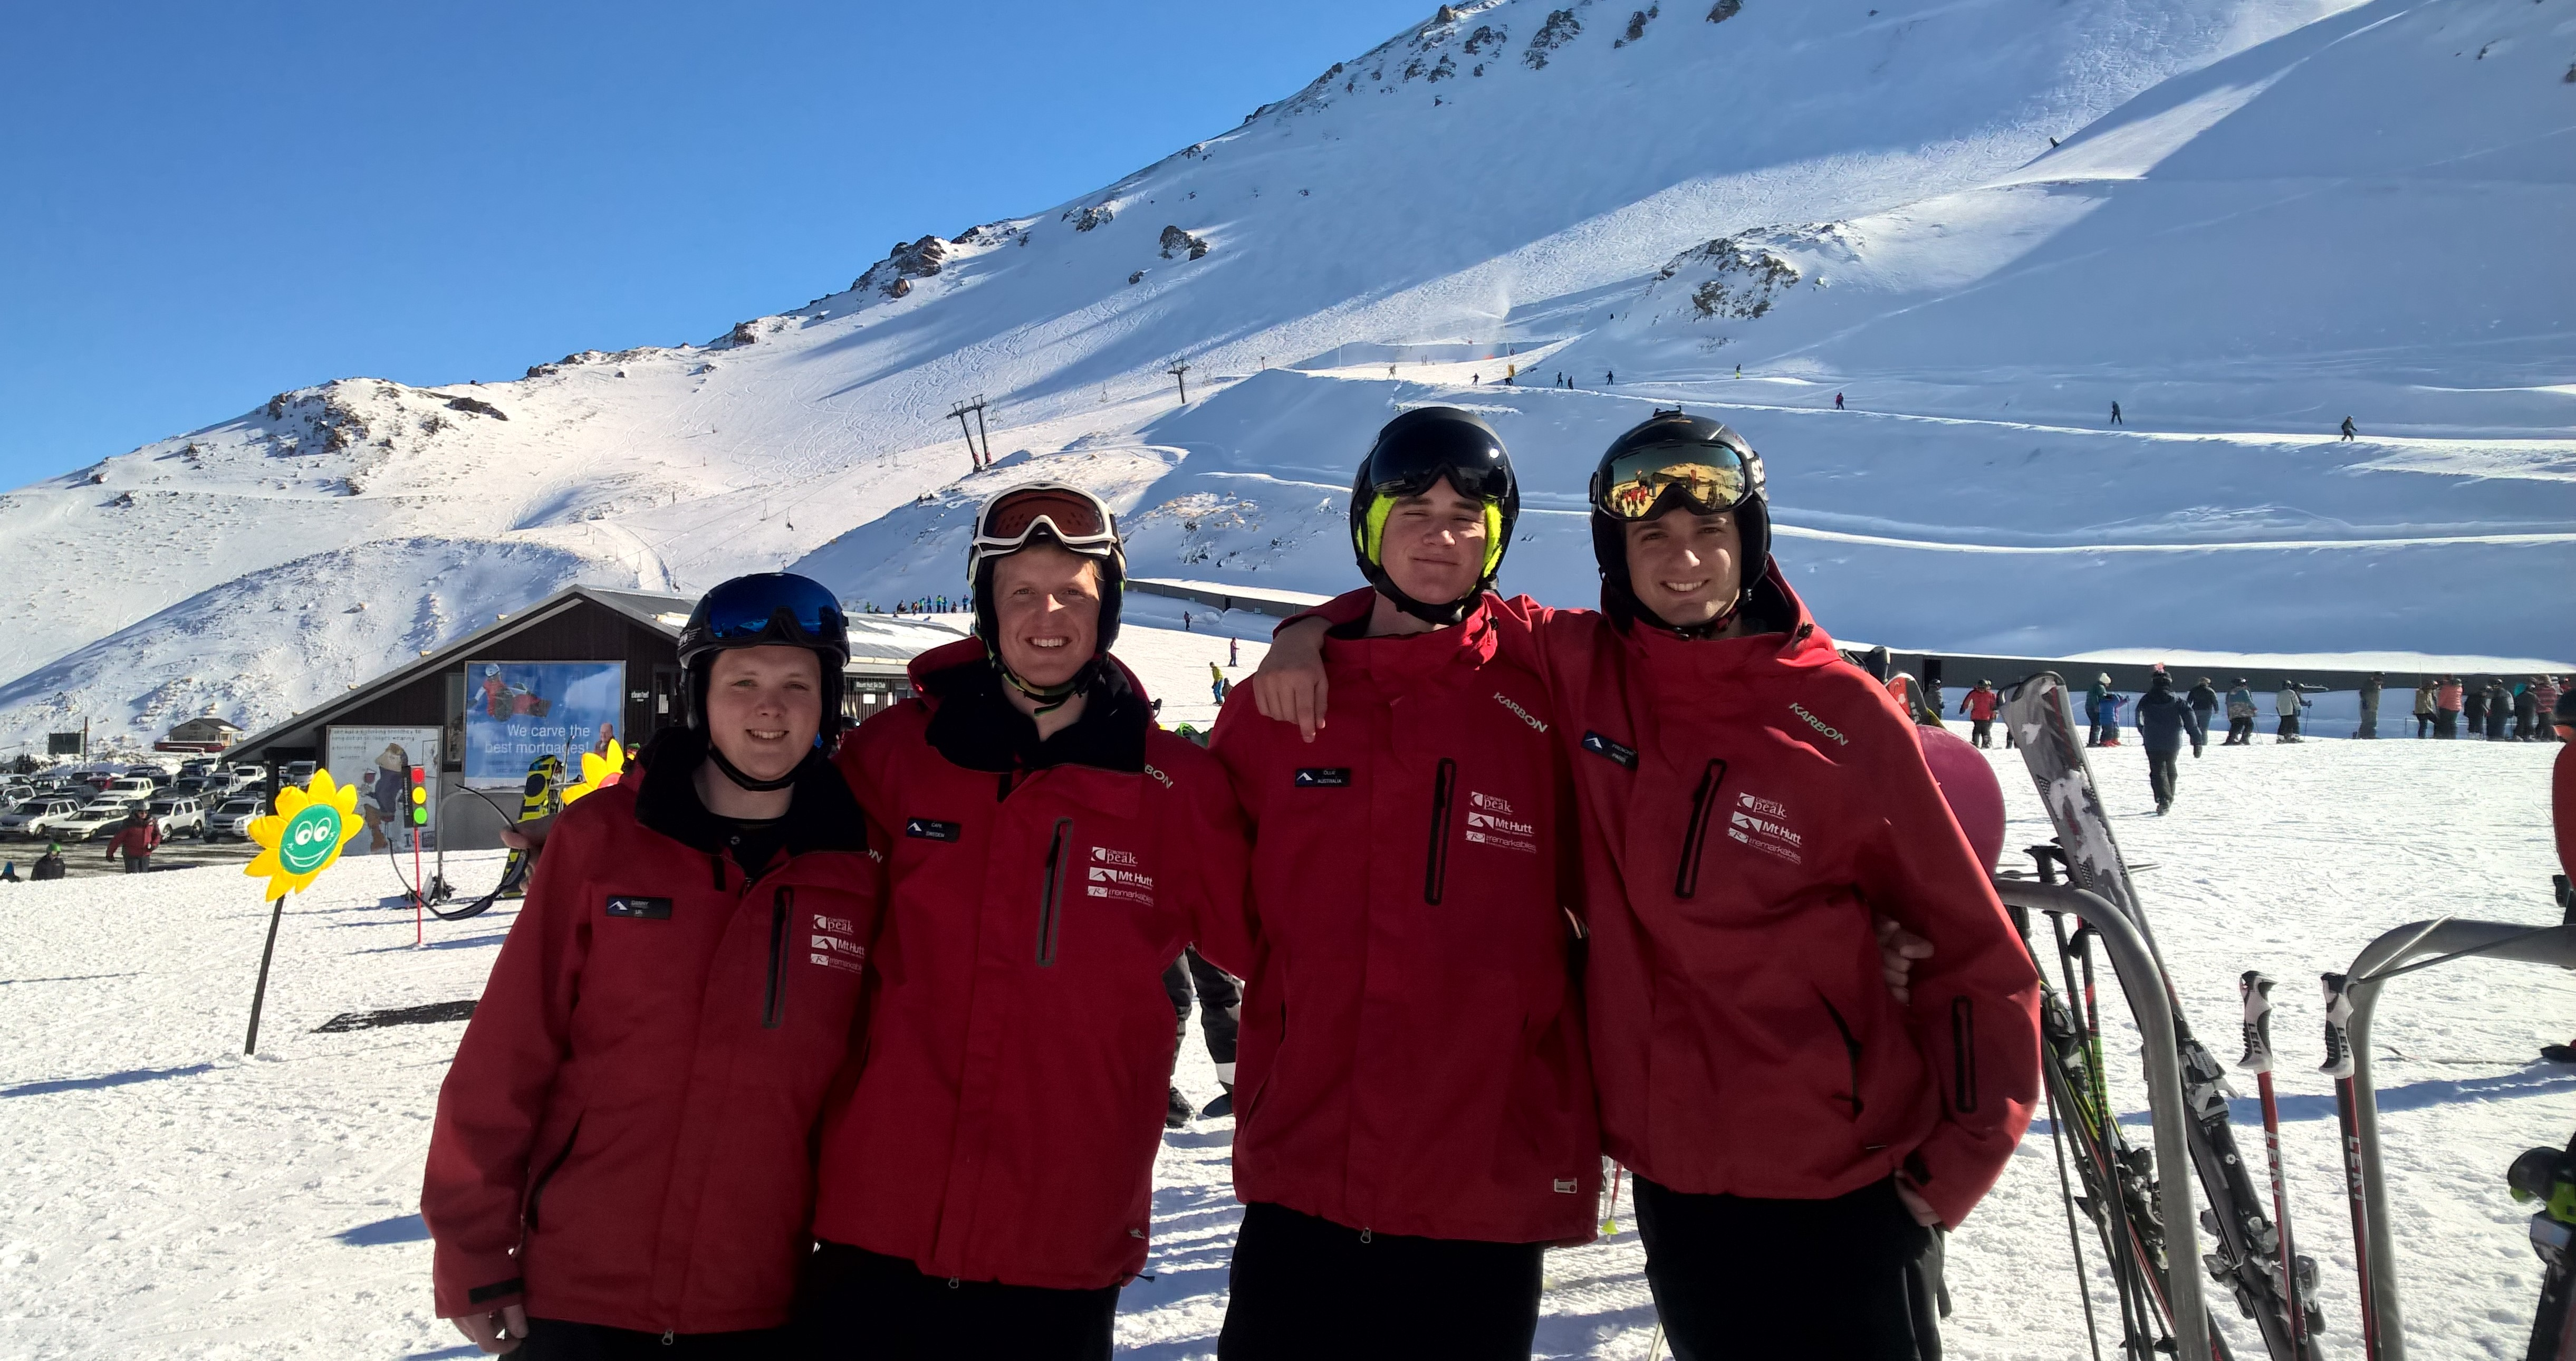
\includegraphics[height=0.4\textwidth]{skiInstructorFriends.jpg}
\end{document}